\section{Theorie}
\label{sec:Theorie}
\subsection{Absorption von \texorpdfstring{$\beta$}{beta}-Strahlung}
Die $\beta$-Strahlung ensteht durch die Umwandlung eines Neutrons in ein Proton, oder eines Protons in ein Neutron und besteht aus Elektronen beziehungsweise Positronen.
Zusätzlich entsteht noch ein Neutrino beziehungsweise Antineutrino.
Dies wird durch folgende Gleichungen beschrieben:
\begin{align*}
  p & \Rightarrow \: n \: + \: {\beta}^{+} \: + \: \nu_\text{e} \\
  n & \Rightarrow \: p \: + \: {\beta}^{-} \: + \: \overline{\nu_\text{e}}
\end{align*}
Die freiwerdende Energie verteilt sich statistisch auf die entstehenden Teilchen.
Das Spektrum eines $\beta$-Strahlers ist somit, wie in Abbildung \ref{fig:betaspektrum}
zu sehen, ein kontinuierliches.
\begin{figure}
  \centering
  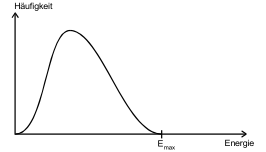
\includegraphics{pictures/betaspektrum.png}
  \caption{Emissionspektrum eines Beta-Strahlers.\cite{sample}}
  \label{fig:betaspektrum}
\end{figure}
Bei der Absoprtion von $\beta$-Strahlung am Festkörper treten eine Vielzahl von Prozessen auf.
Zum einen erleiden die Elek- und Positronen elastische Stoßprozesse. Dies führt zur Rutherfordstreuung.
Dabei werden die $\beta$-Teilchen durch Stöße mit den Atomen im Festkörper beziehungsweise deren Coulomb-Feld gestreut. Dabei kommt es zu keinen großen Energieverlust der Strahlung,
jedoch nimmt die Intensität der Strahlung durch die große Streuung stark ab.
Bei der inelastischen Streuung an den Atomkernen werden die geladenen $\beta$-Teilchen im Coulombfeld der Atome abgebremst und erzeugen sogenannte Bremsstrahlung.
Der Energieverlust durch die Bremsstrahlung ist jedoch für natürliche $\beta$-Strahler relativ gering.
Wesentlich höher ist der Energieverlust durch inelastische Stöße mit den Elektronen des Festkörpers. Dabei treten Ionisations- und Anregungsprozesse an den Atomen auf.
Bei diesen Prozessen verliert das $\beta$-Teilchen zwar nur eine geringe Energiemenge, jedoch treten, vorallem bei Metallen, viele dieser Prozesse hintereinader auf und
bremsen die Strahlung stark ab. Da eine einheitliche analytische Beschreibung unter Berücksichtigung all dieser Absorptionsprozesse sehr schwierig ist, wird im Folgenden
mit empirisch ermittelten Gesetzmäßigkeiten gearbeitet. So zeigt sich grafisch der in Abbildung \ref{fig:betaabsorption} zu sehende Zusammenhang zwischen durchgehender Intensität
und der Massenbelegung $R=\rho D$.
\begin{figure}
  \centering
  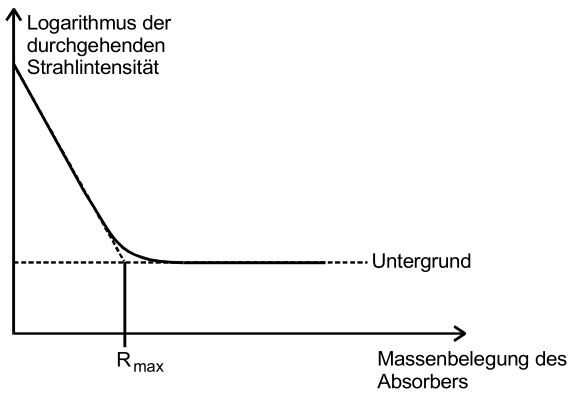
\includegraphics[scale=0.7]{pictures/betaabsorption.png}
  \caption{Schematische Darstellung der Absorptionskurve eines Beta-Strahlers.\cite{sample}}
  \label{fig:betaabsorption}
\end{figure}
Aus dem aus der Grafik \ref{fig:betaabsorption} ermittelten $R_\text{max}$ lässt sich nun die maximale Energie der $\beta$-Strahlung mit
\begin{equation}
  E_\text{max} = 1,92 \sqrt{{R_\text{max}}^2 + 0,22 R_\text{max}} \cdot [\si{\mega\electronvolt}]
  \label{eqn:betaenergie}
\end{equation}
berechnen. $R_\text{max}$ ist dabei in $\si{\gram\per\centi\metre\squared}$ einzusetzen.
